%Marco Teórico
\section{Marco Teórico}
Aproximadamente en el año 1947 se creó el primer transistor y hoy en día se ha convertido en uno de los componentes más útiles y novedosos que podemos encontrar para diversas aplicaciones.

No olvidemos que los transistores iniciaron el camino para la creación de los microprocesadores, los circuitos integrados y las memorias de los computadores.

En la actualidad, la importancia de los transistores en la industria es clave, ya que ofrecen un tipo de tecnología que permite el desarrollo de dispositivos pequeños y muy potentes. Especialmente en aquellas industrias relacionadas con las telecomunicaciones y equipos médicos, entre otras.

\subsection{¿Qué es un transistor BJT?}

\begin{wrapfigure}{r}{0.35\textwidth}
    \centering
    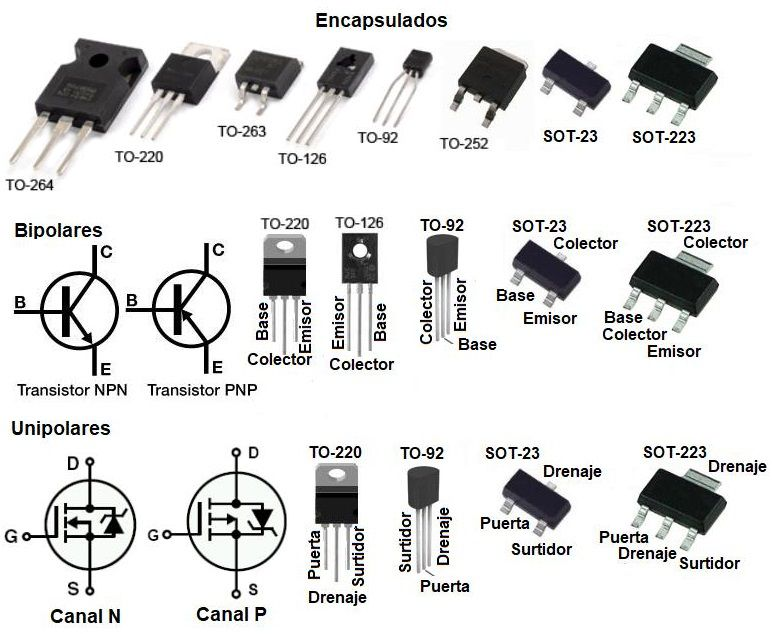
\includegraphics[width=0.35\textwidth]{Imagenes/transistores.jpg}
    \caption{Tipos de transistores}
    \label{fig:transistores}
\end{wrapfigure}

El transistor o BJT es un componente eléctrico semi-conductor que puede ser utilizado para el control adecuado del flujo de corriente eléctrica.


En este caso, una pequeña cantidad de corriente en el conductor base, puede controlar una mayor cantidad de corriente entre el colector y el emisor.

Es por ello que los transistores son muy utilizados en la actualidad para amplificar una señal algo débil (un oscilador o un interruptor, por ejemplo).

En resumen, un transistor puede modificar una señal eléctrica de salida en respuesta a una de entrada, funcionando de esta forma como conmutador, amplificador, rectificador u oscilador.

Entre las características más destacadas de un transistor tenemos:
\begin{itemize}
    \item Es un dispositivo electrónico semiconductor.
    \item Permite el paso de una señal (salida) en respuesta a otra (entrada).
    \item Suelen estar fabricados de cristal de silicio.
    \item Los transistores son sellados herméticamente.
    \item Presentan una carcasa de plástico o una cubierta metálica con tres terminales.
    \item Se puede configurar como amplificador, conmutador, oscilador, o rectificador.
\end{itemize}

\subsubsection{¿Para qué sirven?}

Como ya hemos indicado anteriormente, los transistores son un tipo de dispositivo electrónico que pueden controlar o modificar el flujo de electricidad, siendo ideales para alimentar otros dispositivos pequeños y potentes.

Estos pequeños componentes se elaboran mayormente de silicio y se utilizan en diversos tipos de aparatos electrónicos: teléfonos móviles, tabletas industriales, computadores y robots en las industrias.

Por lo tanto, los transistores tienen diversas aplicaciones en la electrónica y en muchas otras industrias, revolucionado la forma de interactuar entre la tecnología y las actividades cotidianas.
Sin duda, los transistores son un componente muy importante para la industria moderna, ya que permiten circuitos más pequeños y eficientes, y también se pueden usar para diseñar dispositivos digitales de última tecnología.
Adicionalmente, no olvidemos que los transistores pueden ser de tipo “activados o no activados”, y básicamente se diferencian en la forma en que funciona cada uno de ellos.

\subsubsection{¿Cómo funciona un transistor?}
El objetivo principal de un transistor es permitir la transferencia adecuada de energía eléctrica entre las diferentes partes de un circuito eléctrico.

Por lo tanto, los transistores controlan o cambian el flujo de electricidad entre dos puntos, y vienen en muchas formas y tamaños.

Los transistores se utilizan en todo tipo de aparatos electrónicos: desde teléfonos móviles y tabletas, hasta computadores y robots en las industrias.

En términos generales, estos trabajan sobre un flujo de corriente, funcionando como amplificadores al recibir una señal débil y generando una señal más fuerte, o como interruptores al recibir una señal y cortar su paso.

Normalmente, esto ocurre dependiendo de las posiciones que ocupe un transistor en un determinado instante:
\begin{itemize}
    \item \textbf{Posición activa}: aquí se permite el paso de un nivel de corriente variable
    \item \textbf{En corte}: en esta posición no se deja pasar la corriente eléctrica
    \item \textbf{En saturación}: aquí se deja pasar toda la corriente eléctrica (corriente máxima)
\end{itemize}



En cuanto a las partes de un transistor, este se compone de 3 elementos clave: hablamos de la base, colector y emisor.

En ese caso, la base intercede entre el emisor por donde entra la corriente y el colector por donde sale el caudal de corriente.  Es por ello que, si la base de un transistor no recibe corriente eléctrica, este se ubicará en posición de corte. En cambio, si el transistor recibe un flujo de corriente intermedia, la base puede abrir el flujo en una determinada cantidad.

Y, por último, si la base recibe un gran flujo de corriente eléctrica, entonces se abrirá al máximo para pasar el total de la corriente modulada.

Ahora, teniendo un conocimiento previo de lo que es un transistor, se puede saber un poco más sobre como de ese pequeño dispositivo, se puede realizar un análisis detallado de sus configuraciones mas importantes y de ellos crear las etapas que se estudiarán mas adelante.

\subsection{Corrientes del transistor BJT}

Se debe tener en cuenta lo siguiente con las corrientes de los transistores:


\subsubsection{Corriente de colector}
\begin{equation}
    I_C=\beta I_B
    \label{eqn:ic}
\end{equation}
\subsubsection{Corriente de base}
\begin{equation}
    I_B=\dfrac{I_C}{\beta }
    \label{eqn:ib}
\end{equation}
\subsubsection{Corriente de emisor}
\begin{align}
    I_E & =I_B+I_C \label{eqn:ie}                                                                       \\[0.2cm]
    I_E & =\dfrac{I_c}{\beta}+I_C=(\dfrac{1}{\beta}+1)I_C =\dfrac{1+\beta}{\beta}I_C  \label{eqn:ie_ic} \\[0.2cm]
    I_E & = I_B+\beta I_B = I_B(1+\beta) \label{eqn:ie_ib}
\end{align}
\subsection{Configuraciones básicas del BJT}

Los transistores son uno de los componentes más utilizados dentro de la electrónica ya que tienen diferentes configuraciones y polarizaciones, y dependiendo de las variaciones estos funcionan de forma diferente. Cuando se quiere utilizar un transistor como interruptor digital (regiones de corte y saturación) la tarea es fácil ya que el circuito eléctrico es bastante sencillo. En caso de que se utilicé un transistor NPN el emisor se coloca a tierra, el colector a voltaje y la base actúa como interruptor, o si bien se utiliza un transistor PNP se invierten las terminales, el colector a tierra y al emisor se le pone voltaje.

\begin{figure}[H]
    \centering
    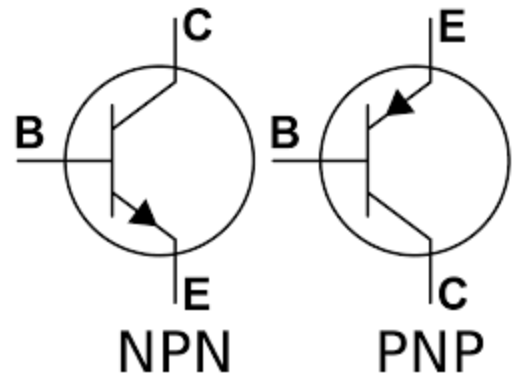
\includegraphics[width=5cm]{Imagenes/simbolo_bjt.png}
    \caption{Símbolo esquemático para cada unos de los transistores BJT}
    \label{fig:simbologia}
\end{figure}

\subsubsection{Emisor Común (EC)}

Esta configuración se utiliza para amplificadores de corriente y voltaje a bajas frecuencias, debido a que tiene una alta ganancia en las dos variables. Una de sus características no tan favorables es que el voltaje de la señal queda invertido en su salida (la corriente no se invierte), es decir las señales quedan como si fueran un espejo. Una forma sencilla de identificar esta configuración es por que la señal de entrada esta en la base y la de salida en el colector. Esta configuración se puede utilizar con todos los tipos de polarizaciones.

\subsubsection{Colector Común (CC)}

Se utiliza para señales con baja potencia y las transforma en el mismo tipo de señal pero con una mayor potencia. Esto se logra por que tiene una alta ganancia de corriente y el voltaje lo transfiere igual ya que no tiene ganancia de voltaje. Otra característica es que en la salida se invierte la corriente. El colector común se utiliza principalmente cuando se requiere poner varios amplificadores conectados en serie debido a que en su entrada tiene mucha impedancia y en su salida disminuye.


\subsubsection{Base Común (BC)} Existen dos formas sencillas de identificar si un transistor esta configurado en base común y estas son; por que el símbolo del transistor se utiliza acostado o porque la entrada es a través del emisor y la salida se encuentra en el colector. A pesar de que esta configuración no tiene una ganancia de corriente se utiliza por que el ancho de banda es más grande que las demás configuraciones y permite trabajar con señales VHF (very high frequency) y UHF (ultra high frequency).


\begin{figure}[H]
    \centering
    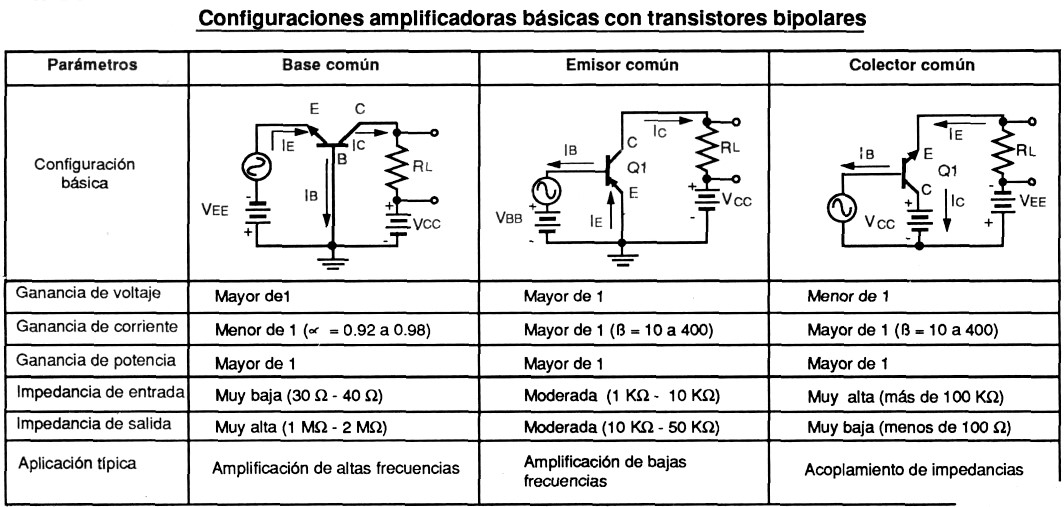
\includegraphics[width=\textwidth]{Imagenes/Configuraciones BJT basicas.jpg}
    \caption{Resumen de configuraciones de los transistores}
    \label{fig:configuraciones}
\end{figure}

Para el cálculo del modelo pi las ecuaciones son distintas
dependiendo su configuración (EC, CC o BC)

\subsection{Polarizaciones de un transistor BJT}

En simples palabras las polarizaciones son circuitos que se utilizan para hacer funcionar a los transistores como amplificadores, en estos circuitos basan su funcionamiento en las configuraciones anteriores, ya que podemos utilizar una de emisor común y utilizar cualquiera de las polarizaciones disponibles todo depende de la aplicación que se le dé al transistor.

\subsubsection{Polarización fija o de base}
Esta polarización solo se puede utilizar con la configuración de emisor común y consiste en colocar una resistencia en la base y una en el colector, mientras que el emisor se conecta a tierra, Al ser una configuración demasiado sencilla tenemos una gran desventaja y es que la señal esta muy expuesta a variaciones dependiendo de los cambios de temperatura que tenga el transistor. Regularmente se utiliza para señales de poca importancia que no importa que se distorsionen.

\subsubsection{Polarización por retroalimentación del emisor o estabilizado en el emisor}
En este tipo prácticamente se le agrega una resistencia en el emisor que hace sea un poco más estable, pero no lo suficiente como para utilizarlo en señales de mucha importancia.

\subsubsection{Polarización por retroalimentación de colector}
Prácticamente se utiliza para regular los cambios de corriente o de voltaje en la fuente de alimentación, ya que si por alguna razón existe una variación, la resistencia que retroalimenta la base actúa para evitar un cambio brusco en la salida del transistor.

\subsubsection{Polarización universal o divisor de voltaje}
Es la más utilizada ya que es la más estable, debido a sus retroalimentaciones. Y si por cualquier razón el transistor se calienta o existen una variación de la corriente la resistencias de retroalimentación actúan para regular la corriente que llega a la base y así poder estabilizar todo el sistema.

\begin{figure}[H]
    \centering
    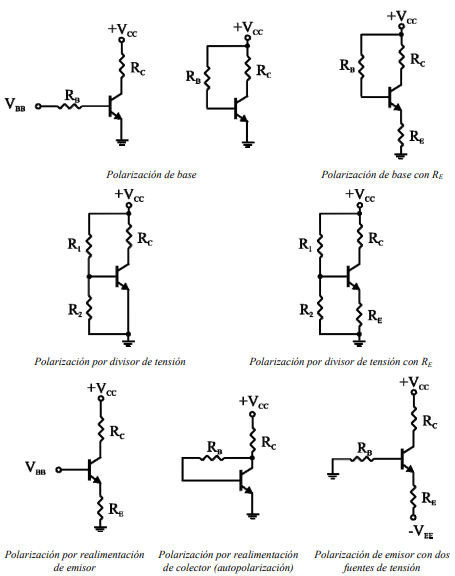
\includegraphics[width=\textwidth]{Imagenes/polarizacion.png}
    \caption{Diferentes circuitos empleados en la polarización de un transistor}
    \label{fig:polarizacion}
\end{figure}

\begin{figure}[H]
    \centering
    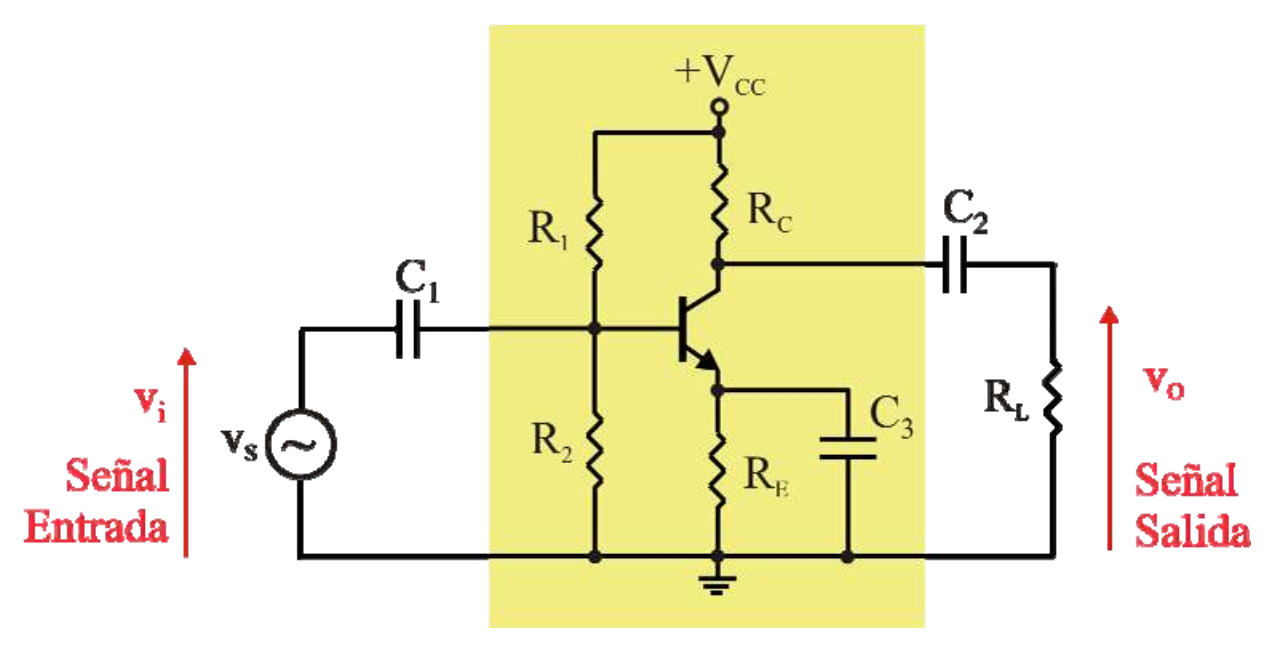
\includegraphics[width=\textwidth]{Imagenes/bjt_ec.png}
    \caption{Circuito amplificador de tensión con BJT en EC}
    \label{fig:ec}
\end{figure}

\subsection{Condensadores de acople y desacople}
En el circuito de la figura \ref{fig:ec} se muestra un circuito típico de un amplificador de tensión con un transistor BJT en emisor común polarizado en la zona activa.
Con él se trata de amplificar una tensión cualquiera vi y aplicarla, una vez amplificada, a una carga que simbolizamos por la resistencia RL. La zona sombreada
resalta el amplificador, que en este caso, lo constituye un transistor BJT en la configuración emisor común. El cual, convenientemente polarizado en la zona activa, es
capaz de comportarse como un amplificador de tensión como ya se mencionó anteriormente.

Los condensadores $C_1$ y $C_2$ que aparecen se denominan condensadores de acoplo y sirven para bloquear la componente continua. En concreto $C_1$ sirve para acoplar la tensión que queremos amplificar al amplificador propiamente dicho, eliminando la posible componente continua que esta tensión pudiera tener. Si no bloqueásemos esta continua se sumaría a las corrientes de polarización del transistor modificando el punto
de funcionamiento del mismo. Por otra parte, el condensador $C_2$ nos permite acoplar la señal amplificada a la carga, eliminando la componente continua (la correspondiente al punto de polarización del transistor) de forma que a la carga llegue únicamente la componente alterna.

El condensador $C_3$ es un condensador de desacoplo, su misión es la de proporcionar un camino a tierra a la componente alterna. En el capítulo anterior se
analizó el efecto de la resistencia $R_E$ desde el punto de vista de su efecto en la estabilización del punto de polarización. Sin embargo, en este capítulo veremos como
desde el punto de vista de la amplificación, esta resistencia hace disminuir la ganancia del amplificador. Al añadir el condensador de desacoplo conseguimos que la continua pase por $R_E$ mientras que la alterna pasaría por el condensador $C_3$ consiguiendo que no
afecte a la amplificación.

\subsection{Principio de superposición}
En este informe vamos a abordar el análisis de este tipo de circuitos amplificadores. Para ello aplicaremos el principio de superposición. En cada punto o rama calcularemos las tensiones y corrientes de continua y de alterna por separado, de forma que al final las tensiones y corrientes finales serán la suma de las calculadas en
cada parte.

Para ello vamos a suponer que el valor de la capacidad de los condensadores, así como la frecuencia de las señales que tenemos es tal que la impedancia que presentan
los condensadores es lo suficientemente pequeña para considerarla nula. Mientras que en continua, estos condensadores presentarán una impedancia infinita. Es decir, consideraremos que en continua los condensadores se comportan como circuitos abiertos (impedancia $\infty$) mientras que en alterna equivaldrán a cortocircuitos (impedancia $0$)

\begin{equation}
    |x_c|=\dfrac{1}{\omega \cdot C}=\dfrac{1}{2\pi f \cdot C}
    \label{eqn:capacitores}
\end{equation}

\begin{figure}[H]
    \centering
    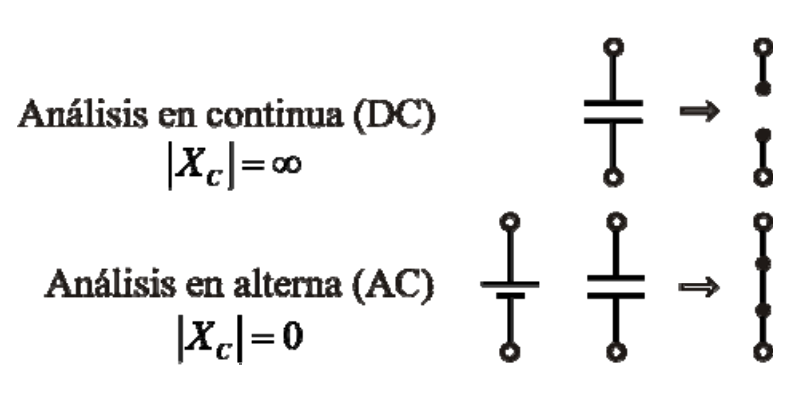
\includegraphics[width=8cm]{Imagenes/analisis_condensadores.png}
    \caption{Consideraciones para aplicar el principio de superposición.}
    \label{fig:consideraciones}
\end{figure}

Aplicando estas consideraciones obtendremos los circuitos equivalentes en DC y en AC que tendremos que resolver separadamente.

Si en el circuito amplificador de la figura \ref{fig:ec} aplicamos la condición de que los condensadores se comportan como circuitos abiertos, obtenemos el circuito equivalente en continua (figura \ref{fig:universal}). Podemos ver como este circuito es, precisamente, el circuito de polarización del transistor cuyo estudio ya se abordó en el punto anterior y de cuya
resolución obtendríamos las tensiones y corrientes de continua presentes en el circuito.

\begin{figure}[H]
    \centering
    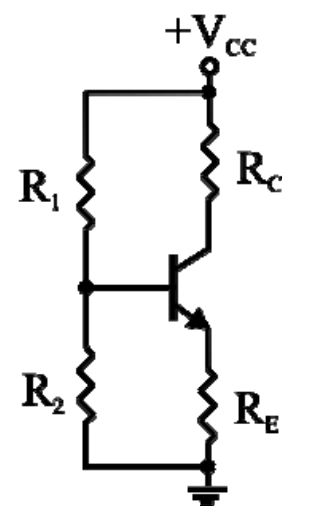
\includegraphics[width=3cm]{Imagenes/universal.png}
    \caption{Circuito equivalente en DC de la figura \ref{fig:ec}}
    \label{fig:universal}
\end{figure}

\subsection{Punto de operación Q}

El punto de operación, es un punto fijo sobre las curvas características, se le conoce también como punto quiesciente (abreviado punto Q). Por definición, quiescente significa quieto, inmóvil, inactivo.

En general, lo importante es calcular los valores de voltajes y corrientes del transistor para una polarización dada. Por tal motivo, se agregara la letra Q a cada
una de los términos que se desean obtener y que son: la corriente de base $I_{BQ}$; la corriente de colector $I_{CQ}$; la corriente de emisor $I_{EQ}$; el voltaje base-emisor $V_{BEQ}$ y el voltaje colector-emisor $V_{CEQ}$. En la mayoría de los casos, la corriente de base $I_{BQ}$ es la primera cantidad que se determina junto con el voltaje base emisor $V_{BEQ}$, una vez que $I_{BQ}$ se conoce, las relaciones de las ecuaciones de malla pueden aplicarse para encontrar las restantes variables como la corriente de colector $I_{CQ}$, etc. Las similitudes en los análisis serán inmediatamente obvias y
las ecuaciones son tan similares para diversas configuraciones que una ecuación
de malla puede derivarse de otra quitando o agregando términos.

\subsection{\texorpdfstring{Modelo $\pi$}{Modelo pi}} %Esta sintaxis es para que no tengo errores al ser referenciado por el entorno hyperref.


\subsubsection{Modelo Pi-híbrido básico del transistor BJT}
Antes de pasar a estudiar el modelo Pi híbrido del transistor voy a compartir un diagrama con la nomenclatura asociada al transistor BJT, con las terminales y las corrientes y voltajes de interés en este dispositivo.

\begin{figure}[H]
    \centering
    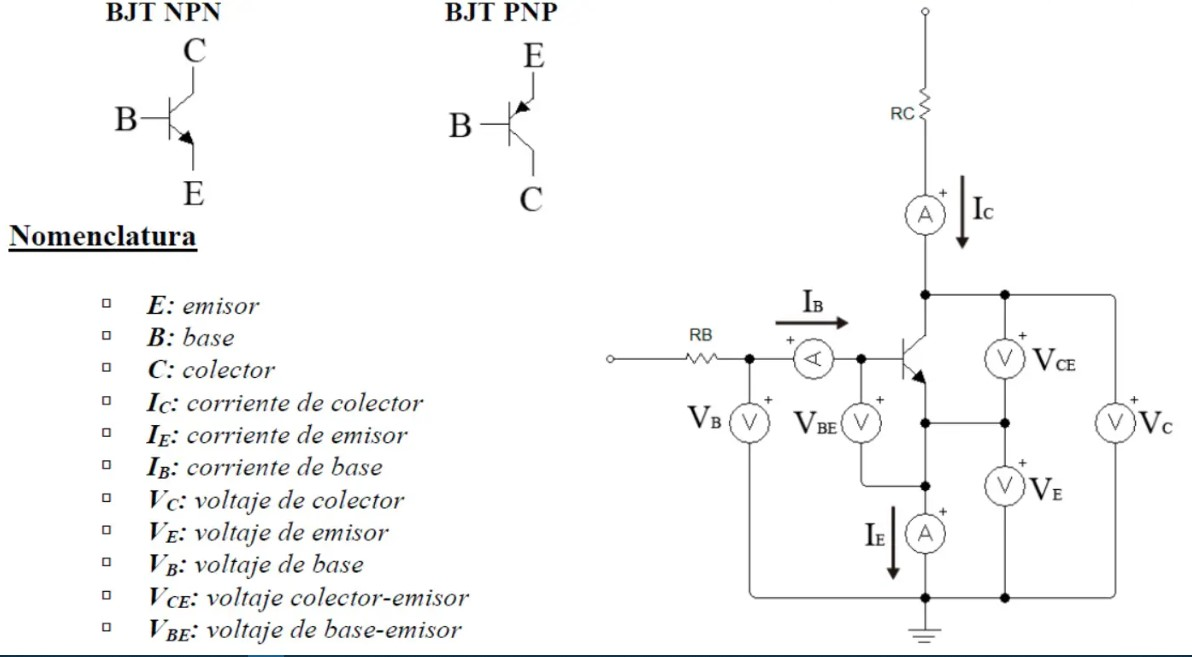
\includegraphics[width=\textwidth]{Imagenes/bjt.jpg}
    \caption{Nomenclatura del BJT}
    \label{fig:bjt}
\end{figure}

Es importante conocer estos términos y como calcularlos, pues de ello dependerá el Modelo Pi. El modelo Pi-híbrido es un modelo de circuito eléctrico que te permite remplazar un transistor en un circuito electrónico por un circuito basado en una fuente dependiente, que facilita el análisis del comportamiento del transistor en condiciones cuando se aplica una señal de frecuencia variable en la entrada del transistor. Básicamente es una convención que permite analizar circuitos con transistores en condiciones de corriente alterna.

Para usar el modelo Pi será necesario remplazar el transistor por un modelo equivalente, el cual se muestra a continuación:

\begin{figure}[H]
    \centering
    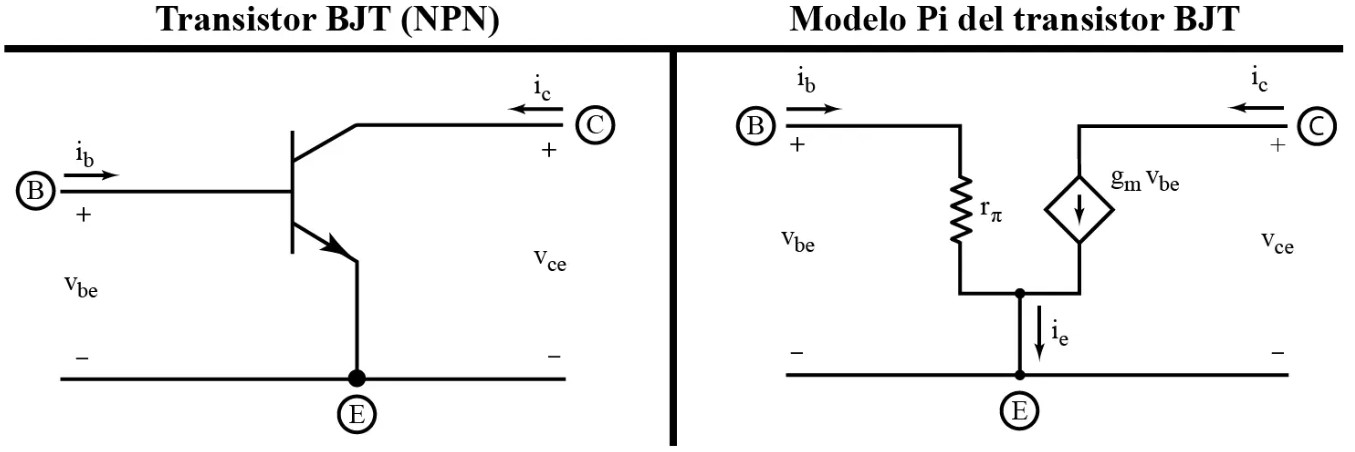
\includegraphics[width=10cm]{Imagenes/modelopi.jpg}
    \caption{Modelo $\pi$}
    \label{fig:modelo_pi}
\end{figure}

Para utilizar el modelo Pi, hace falta calcular dos parámetros: la resistencia $\pi$ y la transconductancia \textbf{$g_m$}. Estos parámetros se calculan utilizando las siguientes ecuaciones:

\begin{gather}
    \mathbf{r_{\pi}} = \dfrac{V_{be}}{i_b} = \dfrac{V_T}{I_{BQ}} = \beta \dfrac{V_T}{I_{CQ}} \label{eqn:rpi}
\end{gather}

\begin{gather}
    \mathbf{g_m}= \dfrac{I_{CQ}}{V_T} \label{eqn:gm}
\end{gather}

En estas ecuaciones la $\beta$ es la ganancia del transistor, la cual es un dato del propio transistor. Este dato casi siempre lo proporciona el enunciado del problema que estemos trabajando. $v_T$ es el voltaje térmico, el cual es aproximadamente 0.026 voltios a la temperatura ambiente (27 ºC). Los sub índices que contienen Q hacen referencia a condiciones de carga.

\subsubsection{Voltaje térmico}

El voltaje térmico ($V_T$) de un transistor bipolar de juntura (BJT) es un parámetro importante que se refiere a la tensión necesaria para mantener una corriente específica en el transistor. Este parámetro es fundamental para entender el comportamiento del transistor en diferentes condiciones de temperatura y corriente.

Se define como la tensión necesaria para mantener una corriente específica en el transistor, usualmente medida entre el colector y la base. Este parámetro es importante porque la temperatura del transistor puede afectar su comportamiento, y el voltaje térmico es una medida de cómo se ajusta la tensión para compensar estos cambios.

\begin{itemize}
    \item Efecto de la temperatura

          Cuando la temperatura del transistor aumenta, la corriente de colector también aumenta debido a que la cantidad de portadores minoritarios en el material semiconductor aumenta. Esto se traduce en un aumento en la corriente de colector. El voltaje térmico se ajusta para compensar este aumento, manteniendo constante la corriente de colector.
    \item Importancia en el diseño

          El voltaje térmico es crucial en el diseño de circuitos que utilizan transistores BJT, ya que permite ajustar la tensión para mantener constante la corriente en diferentes condiciones de temperatura. Esto es especialmente importante en aplicaciones que requieren estabilidad y precisión, como en sistemas de control y amplificación.
\end{itemize}

Siguiendo la siguiente ecuación:

\begin{gather}
    V_T=\dfrac{K \, T}{q}
\end{gather}

Donde, \\
$K$: Constante de Boltzmann $= 1.3806 \, x 10^{-23}$. \\
$q$: Carga del electron $= 1.609 \,x 10^{-19}$. \\
$T$: Temperatura ambiente (en Kelvin) $=25^{\circ} C=298.15 Kelvin$

Teniendo todas las condiciones adecuadas, el valor del voltaje térmico es de $V_T=25.865 m\volt$

\subsubsection{Forma expandida del modelo Pi-híbrido}

El modelo Pi-híbrido expandido toma en cuenta algunos efectos que se producen cuando el transistor opera en condiciones de frecuencia variable y altas frecuencias. A continuación se presenta el modelo Pi-híbrido expandido:

\begin{figure}[H]
    \centering
    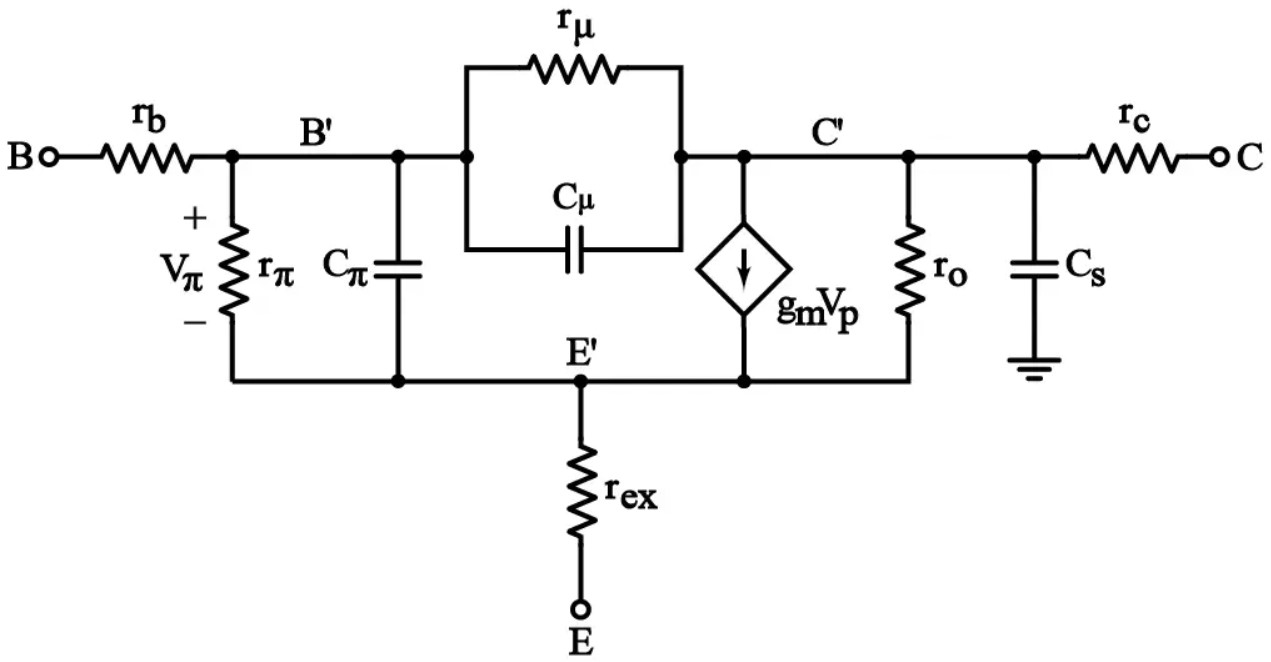
\includegraphics[width=10cm]{Imagenes/modelo pi wh.jpg}
    \caption{Modelo $\pi$ en altas frecuencias}
    \label{fig:modelo_pi_2}
\end{figure}

A continuación procedemos a describir cada uno de los elementos de este modelo:

\begin{itemize}
    \item \textbf{$r_b$, $r_c$, $r_{ex}$:} son resistencias parásitas que se forman en la base, colector y emisor del transistor. Estas resistencias quedan conectadas en serie a las resistencias de base (\textbf{$r_b$}), colector (\textbf{$r_c$}) y emisor (\textbf{$r_{ex}$}). Típicamente poseen valores bajos, entre 1$\Omega$ y 2$\Omega$, por lo cual pueden ser despreciadas.
    \item\textbf{$C_s$:} es la capacitancia del sustrato con el que se construye el transistor. Normalmente posee un valor despreciable. En inglés se conoce como \textbf{junction capacitance of the reverse biased collector–substrate junction}.
    \item\textbf{$C_{\pi}$ y $C_{\mu}$:} son capacitancias asociadas a la juntura del transistor. En inglés se conocen como \textbf{forward-biased junction capacitance o input capacitance} y \textbf{reverse-biased junction capacitance o output capacitance}, respectivamente. Normalmente $C_{\mu}$ es mucho más pequeña que $C_{\pi}$. Sin embargo, por un efecto llamado \textbf{Efecto Miller}, esta capacitancia no puede ser despreciada.

    \item \textbf{$r_\pi$ y $r_{\mu}$:} son resistencias que aparecen en el modelo de corriente alterna. \textbf{$r_{\pi}$} ya la conocemos y sabemos calcularla; \textbf{$r_{\mu}$} es una resistencia con un valor muy alto, típicamente en el orden de los megaohms, por lo cual puede ser despreciada.
\end{itemize}

Algunos de los valores mostrados en el modelo expandido son despreciables por tratarse de resistencias (similar a un circuito abierto) o muy pequeñas (similar a un corto circuito).

\subsubsection{Modelo Pi con efecto Early}

El voltaje Early (denotado por $V_A$) es otro dato del transistor. Es un voltaje que se ubica entre $50$ y $300 V$ y está asociado a la pendiente de las curvas de de polarización del transistor. Este voltaje produce una resistencia denotada por ro que se ubica en la salida del modelo equivalente del transistor, es decir, entre colector y emisor.

\begin{figure}[H]
    \centering
    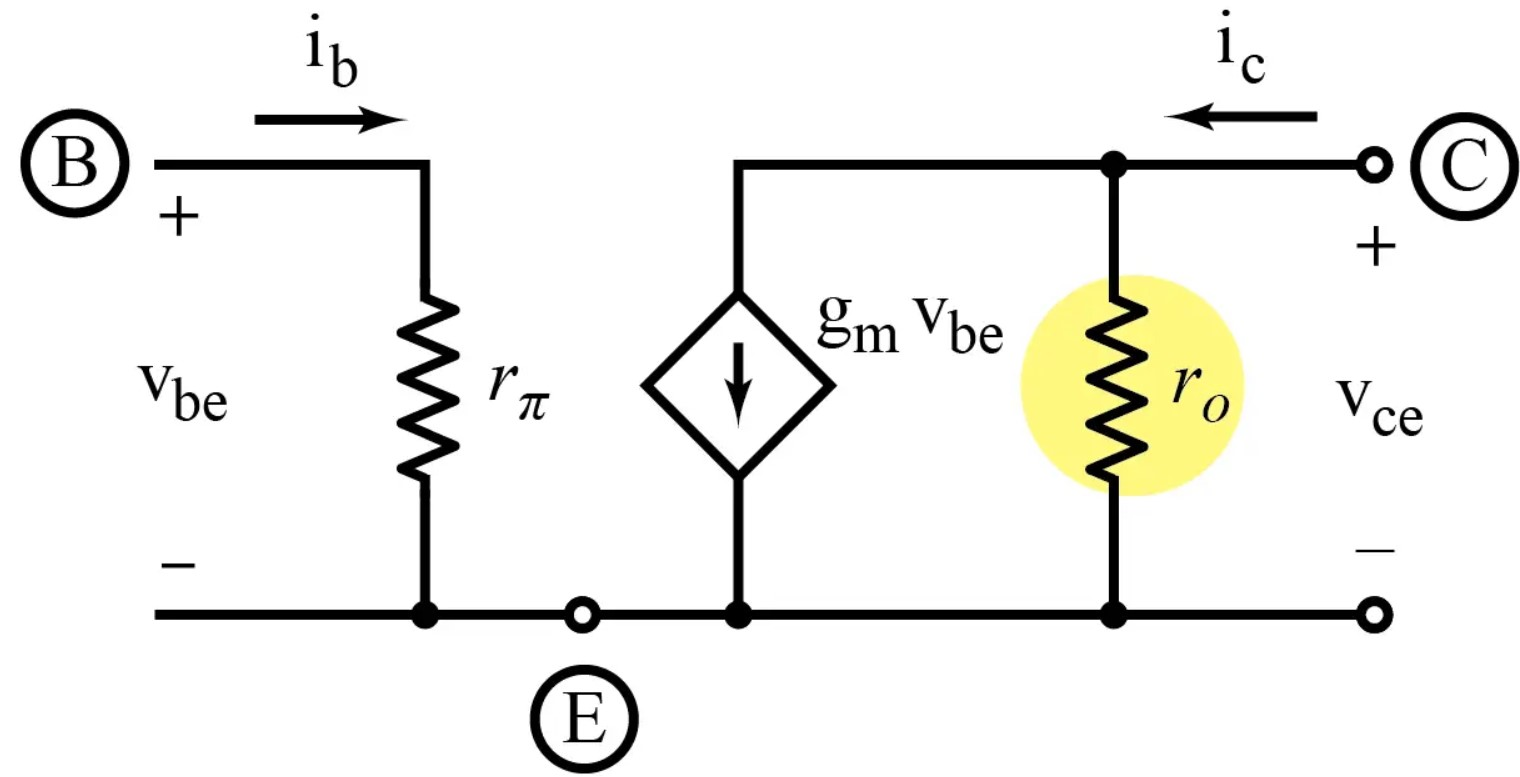
\includegraphics[width=8cm]{Imagenes/modelo_pi3.jpg}
    \caption{Modelo $\pi$ con efecto Early}
    \label{fig:modelo_pi3}
\end{figure}

Para calcular la resistencia $r_o$ se utiliza la siguiente ecuación:

\begin{gather}
    \mathbf{r_o} = \dfrac{V_{A}}{I_{CQ}} \label{eqn:ro}
\end{gather}

Esta resistencia normalmente es de un valor alto, razón por la cual es posible despreciarla. Todo dependerá si se cuenta con un valor de $V_A$, el cual es un dato proporcionado en el enunciado del problema. En otras palabras, es un dato de la hoja de datos del propio transistor.

\subsection{Teorema Miller}

El Teorema de Miller permite redefinir el modelo de corriente alterna del BJT para considerar el efecto de la capacitancia $C_{\mu}$, la cual ya mencionamos en las secciones anteriores de este documento. Sin entrar mucho en detalles, el Teorema de Miller permite hacer lo siguiente:


\begin{figure}[H]
    \centering
    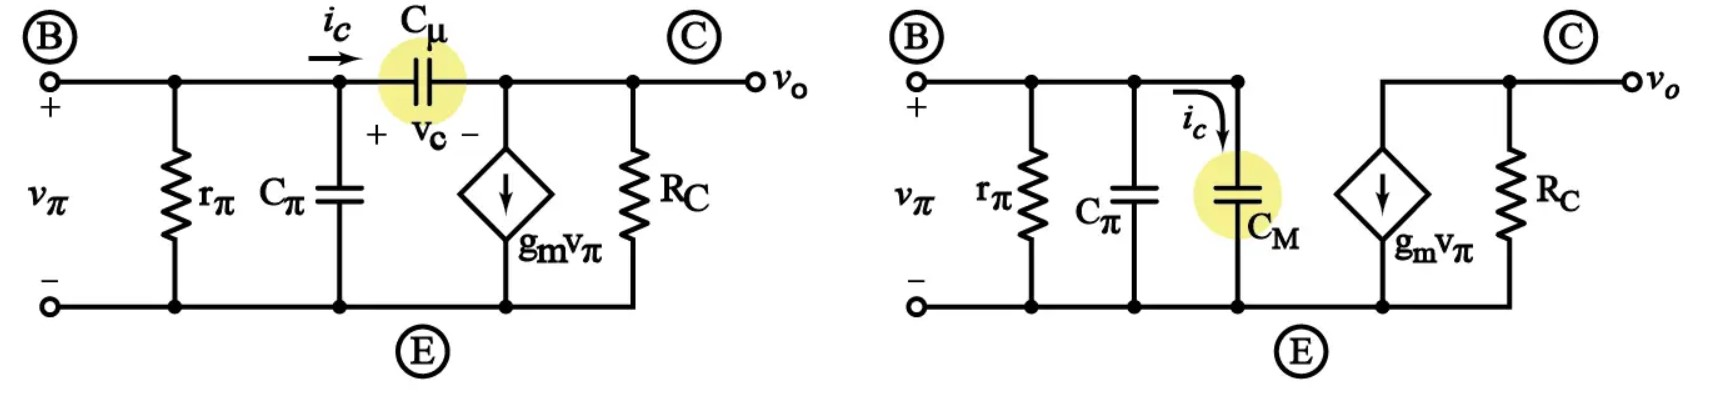
\includegraphics[width=\textwidth]{Imagenes/teorema_miller.jpg}
    \caption{Modelo $\pi$ en altas frecuencias equivalente por el Teorema Miller}
    \label{fig:miller}
\end{figure}

Para hacer la conversión de $C_{\mu}$ a $C_M$ se utiliza la siguiente ecuación:

\begin{equation}
    \mathbf{C_M} =  C_{\pi} + C_{\mu}(1+g_mZ_{out}) = C_{\mu}(1+|A_v|) = \mathbf{C_{eq}} \label{eqn:C_eq}
\end{equation}

En esta ecuación $A_v$ es la ganancia de voltaje del amplificador. Esta ganancia se obtiene al dividir el voltaje de salida entre el voltaje de entrada.

\subsubsection{Resistencia de difusión o intrínseca del emisor ($r_x$)}

$r_x$ en el contexto de transistores bipolares puede referirse a la resistencia de difusión ($r_e$ o resistencia intrínseca del emisor) en el modelo híbrido, no es una nomenclatura estándar comúnmente utilizada en los datasheets de los transistores.

Para calcular la resistencia de difusión se usa la siguiente formula:

\begin{gather}
    r_x=\dfrac{V_T}{I_{E}} \label{eqn:rx}
\end{gather}



\subsection{Ganancia de un amplificador}

Debido a que los amplificadores tienen la capacidad de aumentar la magnitud de una señal de entrada, es útil poder calificar la capacidad de amplificación de un amplificador en términos de una relación salida/entrada. El término técnico para la relación de magnitud salida/entrada de un amplificador es ganancia. Como una relación de unidades iguales (salida de energía/entrada de energía, salida de voltaje/ entrada de voltaje o salida de corriente/entrada de corriente), la ganancia es naturalmente una medición sin unidades.

Matemáticamente, la ganancia está simbolizada por la letra mayúscula “A”.

Las ganancias del amplificador eléctrico se pueden expresar en términos de voltaje, corriente y/o potencia tanto en CA como en CC.

Un resumen de las definiciones de ganancia es el siguiente:

El símbolo “delta” en forma de triángulo ($\triangle$) representa el cambio en las matemáticas, por lo que “$\triangle$V output/$\triangle$V input” significa “cambio en el voltaje de salida dividido por el cambio en el voltaje de entrada”, o más simplemente, “voltaje de salida AC dividido por voltaje de entrada AC”:

\begin{figure}[H]
    \centering
    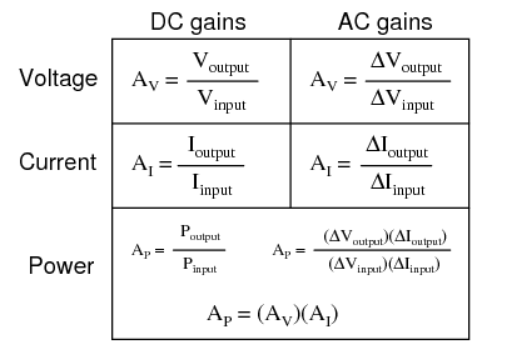
\includegraphics[width=8cm]{Imagenes/gain_amp.png}
    \caption{Distintas Ganancias de un amplificador}
    \label{fig:gain_amp}
\end{figure}

La siguiente ecuación es la mas usada en este capitulo,

\begin{equation}
    A_v=\dfrac{v_o}{V_{in}}
    \label{eqn:av}
\end{equation}





\subsection{Etapas de un amplificador base}
\subsubsection{Amplificador diferencial}
La mayoría de los amplificadores operativos modernos utilizan un extremo frontal de amplificador diferencial. En otras palabras, la primera etapa del amplificador operacional es un amplificador diferencial.

El amplificador diferencial es un circuito que forma parte fundamental de muchos amplificadores y comparadores.

Es un dispositivo que aumenta la diferencia entre dos voltajes de entrada, pero que destruye cualquier voltaje común a dichas entradas. Se trata de un circuito analógico con dos entradas denominadas entrada inversora y entrada no inversora y una sola salida proporcional a la diferencia entre los dos voltajes.

Algunos fabricantes llaman a este instrumento como par diferencial.

En el amplificador diferencial ideal la salida depende de la diferencia de las señales de entrada:

\begin{equation}
    V_o=V_d A_d
\end{equation}

Siendo $V_d$ la señal diferencial y  $A_d$ la ganancia diferencial.

En el amplificador diferencial real la salida depende además de la señal común de ambas entradas:

\begin{equation}
    V_o=V_d A_d+ V_c A_c
\end{equation}

$V_c$ es la señal en modo común
\begin{equation}
    V_c = \dfrac{V_1+V_2}{2}
\end{equation}

$A_c$ es la ganancia en modo común.
A continuación en la figura \ref{fig:diferencial} se muestra la configuración básica de este amplificador.

\begin{figure}[H]
    \centering
    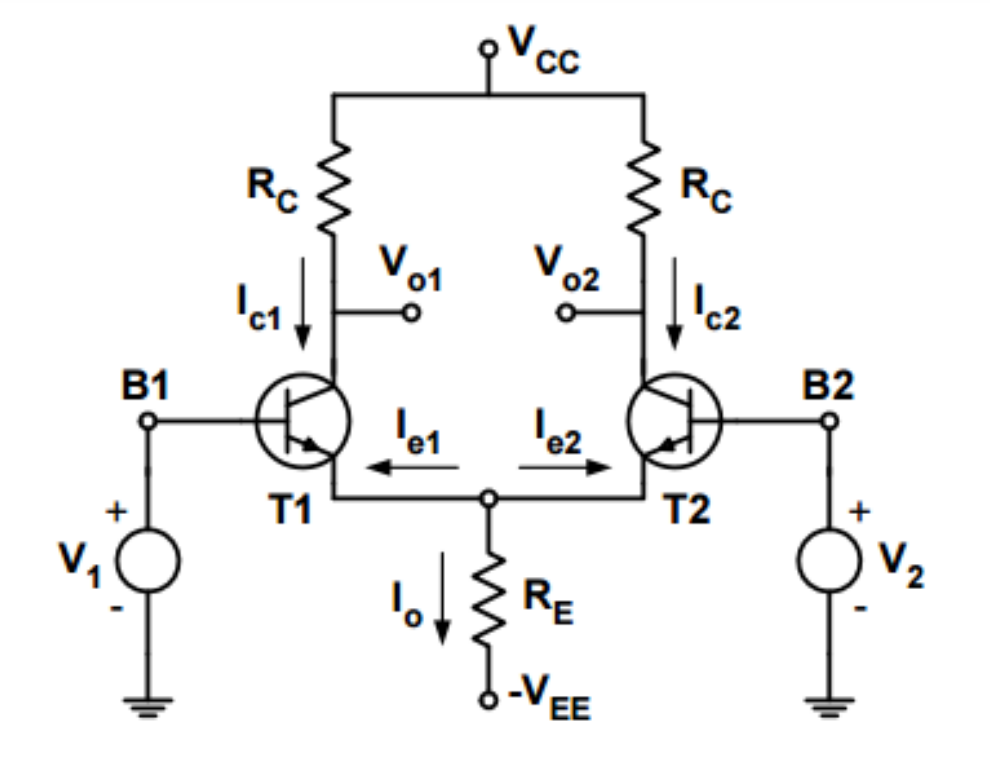
\includegraphics[width=8cm]{Imagenes/diferencial.png}
    \caption{Configuración básica Amplificador Diferencial}
    \label{fig:diferencial}
\end{figure}

Es un montaje simétrico, son dos etapas en emisor común con acoplamiento directo en el emisor.
Las señales de entrada $V_1$ y $V_2$ se aplican en las bases y las señales de salida $V_{o1}$ y $V_{o2}$ se toman en los colectores.
Tenemos:

\begin{align}
    \text{Salida Diferencia:} &  & V_o=V_{o2}-V_{o1} \\
    \text{Salida Asimétrica:} &  & V_o=V_{o2}
\end{align}

\begin{itemize}
    \item \textbf{Ganancia modo diferencial}

          \begin{equation}
              A_d=-\dfrac{V_o}{Z_d}
              \label{eqn:ad}
          \end{equation}


    \item \textbf{Ganancia modo común}

          \begin{equation}
              A_c=-\dfrac{V_o}{Z_c}
              \label{eqn:ac}
          \end{equation}


    \item \textbf{Relación de Rechazo en Modo Común (CMRR)}
          \begin{equation}
              CMRR=\rho=20\cdot log \left| \dfrac{A_d}{A_c}\right|
              \label{eqn:cmrr}
          \end{equation}
\end{itemize}


En la salida diferencial el comportamiento es ideal.
En la salida asimétrica tendremos buen comportamiento si la resistencia $R_E$ es alta ya que con eso conseguimos que $A_c$ sea baja. Cuanto más baja sea $A_c$
más se asemejará al comportamiento ideal.

Para el cálculo de la Relación de rechazo del modo común:

$V_c$ es la señal en modo común

\subsubsection{Amplificador de la etapa elevadora o driver o impulsora}

La etapa de elevación está diseñada para manejar grandes corrientes y voltajes, lo que permite al amplificador operacional manejar cargas pesadas y proporcionar una salida estable y confiable. Esta etapa se compone de transistores bipolares que trabajan en configuración push-pull, lo que significa que un transistor se encarga de manejar la corriente positiva mientras que el otro maneja la corriente negativa. Esto permite una mayor eficiencia y estabilidad en la salida.

La etapa de elevación es fundamental para el funcionamiento del amplificador operacional ya que:

\begin{itemize}
    \item \textbf{Manejo de cargas pesadas}

          La etapa de elevación permite al amplificador operacional manejar cargas pesadas sin perder su capacidad de amplificación.

    \item \textbf{Estabilidad de la salida}

          La etapa de elevación ayuda a mantener la estabilidad de la señal de salida, asegurando que no haya fluctuaciones indeseadas.

    \item \textbf{Amplificación de señales}

          La etapa de elevación es responsable de amplificar la señal de entrada para proporcionar una salida lo suficientemente fuerte para manejar las cargas externas.

\end{itemize}

\subsubsection{Amplificador de potencia}
Un amplificador de potencia es un amplificador electrónico diseñado para aumentar la magnitud de potencia de una señal de entrada.

A diferencia de los amplificadores de voltaje y corriente, un amplificador de potencia está diseñado para impulsar cargas, y se establece como bloque final en un circuito amplificador.

Entre las aplicaciones más frecuentes de un amplificador de potencia destacan:

\begin{itemize}
    \item Medición de valores de impedancia muy bajos.
    \item Medición de impedancia dependiente del voltaje.
    \item Dotar de más potencia en los circuitos durante la medición de impedancia de entrada o de salida.
    \item Generar más energía en entornos ruidosos, como mediciones en convertidores de CC/CC de alta potencia o convertidores de CA/CC.
\end{itemize}

\paragraph{Clases de amplificadores de potencia}

Los amplificadores de potencia más comunes son los que se utilizan en los circuitos de amplificadores de audio y vienen en clases A, B, AB o C.

\subparagraph{Amplificador de potencia clase A:}

En el amplificador de potencia de la clase A, toda la forma de onda de entrada se usa en el proceso de amplificación. Por lo que son los amplificadores de potencia de uso más comunes.

En los amplificadores de potencia de clase A, un único transistor se usa para amplificar las mitades positiva y negativa de la forma de onda. Por otro lado, su ángulo de conducción es de 360º, por lo que los niveles de distorsión de señal son muy inferiores y permiten un mejor rendimiento de alta frecuencia. Sin embargo, una de las principales desventajas de los amplificadores de potencia y especialmente del amplificador de Clase A es que su eficiencia de conversión general es muy baja, ya que las grandes corrientes significan que se pierde una cantidad considerable de energía en forma de calor.

\begin{figure}[H]
    \centering
    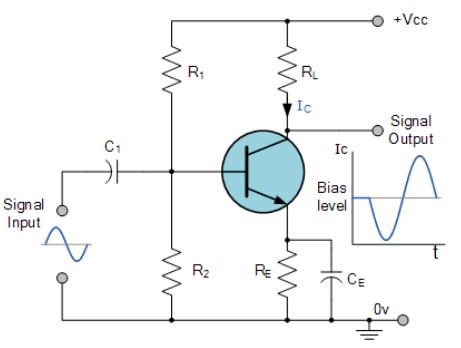
\includegraphics[width=8cm]{Imagenes/potencia_bjt.jpg}
    \caption{Transistor BTJ en configuración Emisor Común para amplificación de CA}
    \label{fig:potencia}
\end{figure}

\subparagraph{Amplificador de potencia clase B o Push and Pull:}

Los amplificadores de Clase B usan dos o más transistores polarizados de tal forma que cada transistor solo conduce durante un medio ciclo (realmente, "casi" medio ciclo) de la onda de entrada. Tienen un rendimiento muy superior a los de Clase A y su diseño no es muy complicado, pero sus aplicaciones se limitan enormemente debido a una característica su propio diseño: una distorsión llamada de "cruce por cero". Aún así, se utilizan incluso en amplificadores que no requieran buena fidelidad y sí facilidad de diseño y rendimiento, como los amplificadores de bocinas y megáfonos de mano.

Para mejorar la eficiencia de potencia total del amplificador de clase A previo, reduciendo la potencia desperdiciada en forma de calor, es posible diseñar el circuito amplificador de potencia con dos transistores en su etapa de salida, produciendo lo que comúnmente se denomina amplificador de clase B; también conocido como configuración de amplificador Push-Pull (empuja-tira en español). Para construir este tipo de amplificador se utilizan necesariamente transistores denominados "complementarios", es decir, de las mismas características eléctricas pero con distintas uniones P-N: si uno es del tipo NPN, el otro ha de ser igual pero de tipo PNP.

\begin{figure}[H]
    \centering
    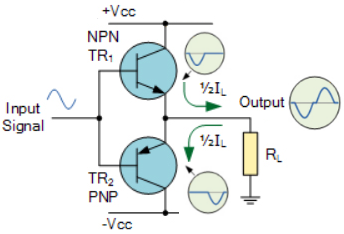
\includegraphics[width=8cm]{Imagenes/clase_b.png}
    \caption{transistores complementarios BJT en funcionamiento clase B, configuración Push-Pull}
    \label{fig:clase_b}
\end{figure}


Los amplificadores Push-Pull utilizan transistores complementarios de potencia, que reciben la misma señal de entrada que es igual en magnitud, pero en fase opuesta entre sí. Esto da lugar a que un transistor solamente amplifica la mitad o 180º del ciclo de la onda de entrada; mientras que el otro transistor amplifica la otra mitad o restante 180º del ciclo de onda de entrada.

Conjuntamente, estas “dos mitades” amplificadas cada una por un transistor, "excitan" o "atacan" la carga o resistencia de salida, dando lugar en ella a la señal completa amplificada.

Por consiguiente, el ángulo de conducción para este tipo de circuito amplificador es escasamente inferior a 180º o $50\%$ de la señal de entrada (para cada transistor). Este efecto de empujar y tirar de los semi ciclos alternos por los transistores da a este tipo de circuito su divertido nombre "push-pull", pero en general se lo conoce como el amplificador de clase B.

Realmente los transistores en un amplificador de clase B no llegan al conducir el $50\%$, ya que ambos necesitan tener una polarización al menos de 0.65 V Emisor-Base para empezar a conducir y amplificar. Esto supone que de la señal de entrada, en los primeros 0.65 V. (positivos y negativos), la señal de salida va a estar a "0". Y sólo cuando en la entrada se superen los 0.65 V. E-B podrá empezar a amplificar la salida. Esto, al final, produce inevitablemente una falta de amplificación en torno a los valores cercanos a "0" V. denominada "distorsión de paso por cero" o "distorsión de cruce", característica de los amplificadores en Clase B.

\begin{figure}[H]
    \centering
    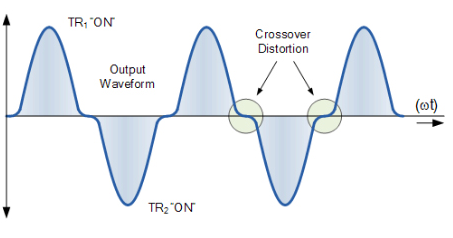
\includegraphics[width=10cm]{Imagenes/crossover.png}
    \caption{formas de señal de saldia debida a la "distorsión de cruce"    o     "de paso por 0" en un amplificador Clase B, Push-Pull}
    \label{fig:crossover}
\end{figure}

\subparagraph{Amplificador de potencia clase AB:}

Un amplificador de clase AB está polarizado de modo que la corriente de salida fluye durante menos de un ciclo completo de la forma de onda de entrada pero más de medio ciclo. La implementación de los amplificadores de Clase AB es muy similar a las configuraciones de Clase B estándar en que utiliza dos transistores de conmutación como parte de una etapa de salida complementaria con cada transistor conduciendo en semi-ciclos opuestos de la forma de onda de entrada antes de combinarse en la carga.

Por lo tanto, al permitir que ambos transistores de conmutación conduzcan corriente al mismo tiempo durante un período muy corto, la forma de onda de salida durante el período de cruce cero se puede suavizar sustancialmente reduciendo la distorsión de cruce asociada con el diseño del amplificador de clase B. Entonces el ángulo de conducción es mayor de 180° pero mucho menor de 360°.

\begin{figure}[H]
    \centering
    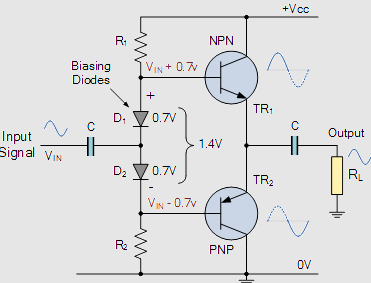
\includegraphics[width=10cm]{Imagenes/clase_ab.png}
    \caption{Esquemático de un amplificador clase AB, polarizado por diodos }
    \label{fig:clase_ab}
\end{figure}

Una configuración de amplificador de clase AB es más eficiente que un amplificador de clase A pero un poco menos eficiente que la de un clase B debido a la pequeña corriente de reposo necesaria para polarizar los transistores justo por encima del límite. Sin embargo, el uso de polarización incorrecta puede causar picos de distorsión cruzada que producen una peor condición.

Dicho esto, los amplificadores de clase AB son uno de los diseños de amplificadores de potencia de audio más preferidos debido a su combinación de una eficiencia razonablemente buena y una salida de alta calidad, ya que tienen una baja distorsión de cruce y una alta linealidad similar al diseño de amplificador de clase A.

\subparagraph{Amplificador de potencia clase C:}

Los amplificadores de potencia en clase C parten de la premisa siguiente: no se trata de amplificar con calidad la señal de entrada, se trata simplemente de amplificar la señal de entrada de modo que a la salida se obtenga el máximo rendimiento posible pero sólo para un rango de frecuencias muy reducido, en torno a una de "resonancia".

Son amplificadores que desde luego no sirven para señales de audio, por la distorsión. Su campo de aplicación está en las telecomunicaciones, en radiofrecuencia, F, donde se requiere un incremento en el nivel de potencia y no se requiere linealidad entre la tensión de entrada y tensión de salida. Los amplificadores Clase C pueden ser modulados en amplitud para amplificar una portadora modulada en frecuencia.

\begin{figure}[H]
    \centering
    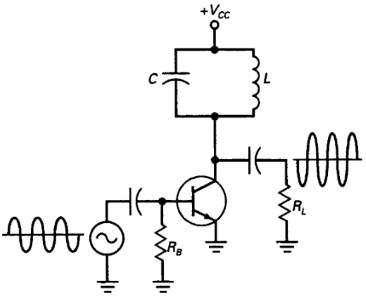
\includegraphics[width=7cm]{Imagenes/amplificador resonante01.png}
    \caption{etapa amplificadora a transistor BJT con circuito tanque resonante }
    \label{fig:clase_c}
\end{figure}

Este tipo de amplificadores se reconoce porque tienen, en lugar de la resistencia de colector típica, un "circuito tanque" formado por un condensador y bobina diseñados para que en un estrecho margen de frecuencias entren en sintonía -por lo que también se le llama "circuito resonante"-y, modificando la impedancia del circuito L-C produzcan la conducción del transistor. Es por eso que a este tipo de circuitos les llama amplificadores "resonantes" o "sintonizados".

En torno a la frecuencia de resonancia, estos amplificadores obtienen una ganancia alta; fuera de esta frecuencia, la amplificación es muy reducida y el consumo es mínimo.


\begin{figure}[H]
    \centering
    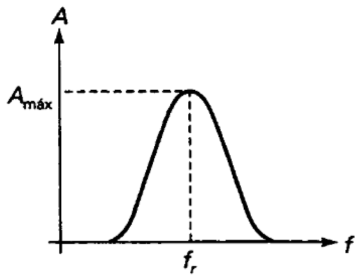
\includegraphics[width=7cm]{Imagenes/amplificador resonante02.png}
    \caption{etapa amplificadora a transistor BJT con circuito tanque resonante }
    \label{fig:campana de gauss}
\end{figure}

\subsubsection{Amplificadores de varias etapas}

La conexión más utilizada para amplificadores de varias etapas:

\paragraph{\textbf{Conexión en cascada}}

\begin{figure}[H]
    \centering
    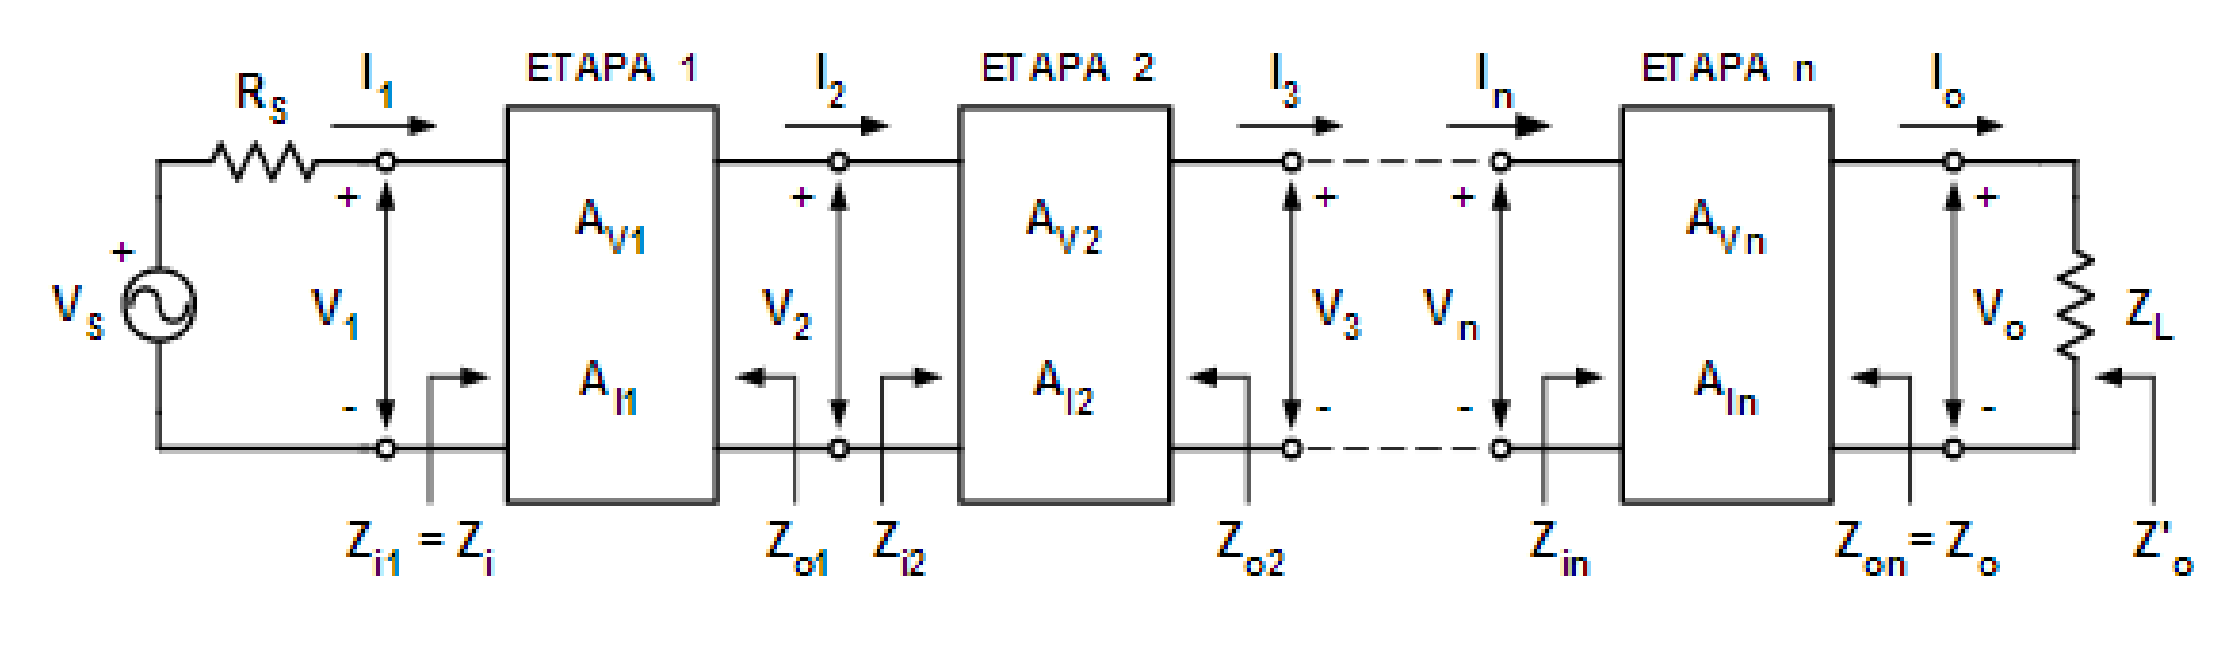
\includegraphics[width=15cm]{Imagenes/amp_base.png}
    \caption{Conexión en cascada de varios amplificadores}
    \label{fig:cascada}
\end{figure}

Hay influencias de una etapa sobre otra, la señal de salida de cada etapa se aplica como señal de entrada de la siguiente.

Las ganancias de tensión de cada etapa y sus impedancias teniendo en cuenta lo siguiente, serán:
\begin{gather}
    A_v= A_{v1}A_{v2}...A_{vn}
    \label{eqn:avt}
\end{gather}

\begin{align*}
     & \text{Impedancia de entrada} &  & Z_in= Z_n        \\
     & \text{Impedancia de salida}  &  & Z_o= Z_{On}      \\
     &                              &  & Z'_o= Z_{L}||Z_o
\end{align*}

Nosotros nos centraremos en los amplificadores de alterna, hay varios tipos de acoplamientos entre etapas, aquí nos centraremos en el acoplamiento RC.

El acoplamiento entre etapas es mediante un condensador. Como se indico anteriormente sobre los condensadores de acople y desacople.

\newpage

\subsection{Respuesta en frecuencia}

A respuesta en frecuencia de un amplificador operacional en lazo cerrado o lazo abierto se define como el límite de alta frecuencia y el límite de baja frecuencia. En estos límites, la ganancia de voltaje se reduce un 0.707 del valor máximo de voltaje, en el rango de frecuencia útil.
El ancho de banda para pequeña señal es la diferencia entre el límite de alta frecuencia y el límite de baja frecuencia. Además se debe agregar que:

\begin{itemize}
    \item \textbf{Para frecuencias medias}, los condensadores de acople y desacople se comportan como un cable, es decir, un cortocircuito.
    \item \textbf{Para frecuencias altas}, las limitaciones en frecuencia de los dispositivos activos condicionan 1a frecuencia máxima de operación del amplificador.
    \item \textbf{Para frecuencias bajas}, el efecto de los condensadores de acoplo y desacoplo es importante.
\end{itemize}

\subsubsection{Análisis de respuesta en frecuencia}

\begin{itemize}
    \item \textbf{Frecuencias bajas:} Se toma en cuenta el condensador que se va a estudiar en bajas frecuencias, siendo estos los de acople, desacople y bypass. Al escoger el condensador, ese se reemplaza por una fuente de prueba y los demás capacitores se cortocircuitan y los de alta frecuencia son un abierto. Así, se puede hallar la impedancia equivalente. Se hace uso de la ecuación \ref{eqn:wl}.

          \begin{equation}
              w_{p_n}=\dfrac{1}{C_nZ_{eq}}
              \label{eqn:wl}
          \end{equation}

    \item \textbf{Frecuencias altas:} Se toma en cuenta los capacitores que estén conectados entre base y emisor o base y colector, con un valor de capacitancia bastante bajo, cercano a los $\si{pF}$. Se aplica el teorema de miller, que es la ecuación \ref{eqn:C_eq} y su frecuencia de corte superior siendo la ecuación \ref{eqn:wh}.

          \begin{equation}
              w_{H}=\dfrac{1}{C_{eq}Z_{in}}
              \label{eqn:wh}
          \end{equation}

    \item \textbf{Frecuencia de corte superior total}
          \begin{equation}
              w_t=\beta \cdot f_H
              \label{eqn:wt}
          \end{equation}
\end{itemize}



\subsection{Realimentación en un amplificador}

La realimentación consiste e11 combinar una muestra de la señal de salida del amplificador con la señal de entrada, de modo tal que se modifican las características generales del sistema. Puede ser positiva o negativa.

\subsubsection{Realimentación negativa}

La realimentación es negativa cuando el valor de la señal de salida es menor que sin la realimentación. Para ello, la serial de salida que se toma como muestra es aplicada opuesta en fase a la serial de entrada.

La realimentación negativa disminuye la ganancia del amplificador y a pesar de ello, la inmensa mayoría de los amplificadores utilizan esta variante de realimentación debido a las muchas ventajas que se obtienen con la aplicación de este principio, tales como el aumento
de la estabilidad y el ancho de banda, 1a disminución de las distorsiones de frecuencia y de no linealidad así como del ruido y el cambio en las resistencias de entrada y salida. Todo esto incrementa notablemente la calidad y versatilidad de los amplificadores.

Los cambios provocados por el envejecimiento de los componentes y dispositivos, su reemplazo u otras causas, las variaciones de temperatura, etcétera, se reflejan en las alteraciones que puede sufrir la ganancia de un amplificador con relación a su valor original. Tales
alteraciones son de hecho reducidas con la realimentación negativa, a tal extremo que su ganancia puede llegar a depender solamente de las características de la red de realimentación, cuando la ganancia de lazo es mucho mayor que la unidad.


\subsubsection{frecuencia de corte inferior en realimentación no inversora}
\begin{equation}
    w_{L_{fb}}=\dfrac{w_L}{A_{fb}}=\dfrac{w_L}{1+\dfrac{R_f}{R_s}}
    \label{eqn:wlfb}
\end{equation}
\subsubsection{frecuencia de corte superior en realimentación no inversora}
\begin{equation}
    w_{H_{fb}}=w_H(A_{fb})=w_L(1+\dfrac{R_f}{R_s})
    \label{eqn:whfb}
\end{equation}

\subsubsection{Ganancia en retroalimentación de un no inversor}
\begin{equation}
    A_{fb}=1+\dfrac{R_f}{R_s}
    \label{eqn:afb}
\end{equation}


\subsubsection{Impedancias de entrada en realimentación negativa o degenerativa}
\begin{equation}
    Z_{in}=Z_d\left(1 +\dfrac{A_{fm}}{A_{fb}}\right)
    \label{eqn:zinfb}
\end{equation}
\subsubsection{Impedancias de salida en realimentación negativa o degenerativa}
\begin{equation}
    Z_{o}=\left(\dfrac{Z_o}{\dfrac{A_{fm}}{A_{fb}}}\right)
    \label{eqn:zofb}
\end{equation}
\subsubsection{Realimentación positiva}

La realimentación es positiva cuando el valor de la señal de salida es mayor que sin la realimentación. Esto se logra cuando la señal de salida que se toma como muestra es
aplicada en fase con la señal de entrada.

El resultado de la realimentación positiva es contrario a la realimentación negativa, es decir se incrementa el ruido, la ganancia y la distorsión, disminuyendo el ancho de banda y la estabilidad, por lo cual este efecto no es aconsejable para los amplificadores, sin embargo, puede ser aprovechado con gran eficacia en los circuitos osciladores.

\subsection{Método de amplificador desvanecido}

El método consiste en añadir una ganancia adicional variable a la señal recibida, dependiendo de la calidad de la señal, para compensar la atenuación y mejorar la relación señal—ruido. Esta ganancia adicional se calcula en función de la retroalimentación recibida de la señal de error, que se obtiene comparando la señal recibida con la señal transmitida originalmente.

El Amplificador Desvanecido puede ser implementado de varias maneras, incluyendo la retroalimentación de la señal de en un circuito de control de ganancia, o utilizando
técnicas de procesamiento digital de señales para ajustar la ganancia en tiempo real.

Este método es particularmente útil en sistemas de comunicación inalámbrica de alta frecuencia, como los sistemas de comunicación móvil, donde la atenuación de la señal debido a la propagación en el medio ambiente puede ser significativa y afectar la calidad de la señal
recibida.

\subsection{Método de Blackman}

Es una técnica utilizada para calcular la impedancia de entrada de un amplificador.Esta técnica se basa en la medición de la tensión de entrada y corriente de entrada del
amplificador, y en el uso de una red de resistencias y capacitores para modelar la impedancia
de entrada del amplificador.

El método de Blackman utiliza una red de dos resistencias y un capacitor, conectados en serie con la entrada del amplificador. La tensión de entrada se mide a través de una de las resistencias, mientras que la corriente de entrada se mide a través de la otra resistencia.

A partir de estas mediciones, se puede calcular la impedancia de entrada del amplificador utilizando la ley de Ohm y la ley de Kirchhoff.

La ventaja del método de Blackman es que permite obtener una medida precisa de la impedancia de entrada del amplificador en una amplia gama de frecuencias. Además, esta
técnica es relativamente sencilla y económica de implementar, lo que la hace adecuada para su uso en aplicaciones practicas.

Sin embargo, es importante tener en cuenta que el método de Blackman asume que la impedancia de entrada del amplificador es constante en toda la gama de frecuencias de
interés, lo cual puede no ser cierto en algunos casos.

\subsection{Formula de propagación de incertidumbres}

Para calcular la incertidumbre en un resultado calculado indirectamente, como \( V_{CE} = V_C - V_E \), puedes utilizar la fórmula de propagación de incertidumbres. Esta fórmula se aplica cuando tienes dos o más cantidades medidas y deseas determinar la incertidumbre en una cantidad derivada a partir de ellas. La fórmula general es:

\[ \Delta Q = \sqrt{\left(\frac{\partial Q}{\partial A} \Delta A\right)^2 + \left(\frac{\partial Q}{\partial B} \Delta B\right)^2 + \ldots} \]

Donde:
- \( Q \) es la cantidad derivada (en este caso, \( V_{CE} \)),
- \( A, B, \ldots \) son las cantidades medidas (en este caso, \( V_C \) y \( V_E \)),
- \( \Delta A, \Delta B, \ldots \) son las incertidumbres asociadas a las cantidades medidas, y
- \( \frac{\partial Q}{\partial A}, \frac{\partial Q}{\partial B}, \ldots \) son las derivadas parciales de \( Q \) con respecto a \( A, B, \ldots \).

En este caso, como \( V_{CE} = V_C - V_E \), las derivadas parciales son simples:

\[ \frac{\partial V_{CE}}{\partial V_C} = 1, \quad \frac{\partial V_{CE}}{\partial V_E} = -1 \]

Entonces, la fórmula para la incertidumbre en \( V_{CE} \) sería:

\[ \Delta V_{CE} = \sqrt{\left(\Delta V_C\right)^2 + \left(\Delta V_E\right)^2} \]

Sustituyendo los valores dados:

\[ \Delta V_{CE} = \sqrt{(0.1)^2 + (0.02)^2} \]

\[ \Delta V_{CE} = \sqrt{0.01 + 0.0004} \]

\[ \Delta V_{CE} \approx \sqrt{0.0104} \]

\[ \Delta V_{CE} \approx 0.102 \volt \]

Entonces, la incertidumbre en \( V_{CE} \) es aproximadamente \( \pm 0.102 \volt \). Puedes informar el resultado como \( V_{CE} = 1.06 \pm 0.102 \volt \).

\subsection{Error Porcentual}

Porcentaje de error (\% de error), también conocido como porcentaje de error, es una medida de cuánto un valor difiere del valor esperado. Puede usarse para determinar qué tan lejos está un valor esperado de otro valor, pero a menudo se usa en el contexto de experimentos científicos.

Se puede expresar en la siguiente ecuación:

\begin{equation}
    E_r =\dfrac{|Valor_{experimental}-Valor_{teorico}|}{Valor_{teorico}} \cdot  100
    \label{eqn:error}
\end{equation}

\subsection{Impedancia de entrada/diferencial (medición indirecta)}

La siguiente ecuación se lleva a cabo debido a un divisor de tensión realizado de la siguiente manera:

\begin{figure}[H]
    \centering
    \begin{circuitikz}[transform shape,scale=1]

  \draw (2.25,-2.25) to[short,-*] (2.25,-2.25) coordinate (X0);
  \def\OpAmpsopamp(#1)#2#3{%
    \begin{scope}[#1,transform canvas={scale=1}]
      \draw (0.0,0.25) -- (1.0,-0.25);
      \draw (0.0,-0.75) -- (1.0,-0.25);
      \draw (0.0,0.25) -- (0.0,-0.75);
      \draw (0.0625,0.0) -- (0.1875,0.0);
      \draw (0.0625,-0.5) -- (0.1875,-0.5);
      \draw (0.125,-0.5625) -- (0.125,-0.4375);
      \draw (0.5,0.25) coordinate (#2 text);
      \draw (0.0,0.0) coordinate (#2 X0);
      \draw (0.0,-0.5) coordinate (#2 X1);
      \draw (1.0,-0.25) coordinate (#2 X2);
    \end{scope}
    \draw (#2 text) node[right] {#3};
  }
  \draw (2.25,-3.5) node[ground] {} ;
  \node[right] at (-2.0,-2.25) {Vg} ;
  \node[right] at (2,-2.0) {Vi} ;
  \node[right] at (5.5,-2.5) {Vo} ;
  \OpAmpsopamp (shift={(3.5,-2.25)},rotate=0  ) {B0} {Amp. Op};
  \draw (X0) to[R,l=Rp] (-0.5,-2.25) ;
  \draw (B0 X0) to[short,-] (X0) ;
  \draw (5.5,-2.5) to[short,-] (5.0,-2.5) ;
  \draw (B0 X1) to[short,-] (2.25,-2.75) ;
  \draw (2.25,-3.5) to[short,-] (2.25,-2.75) ;
  \draw (-0.5,-2.25) to[short,-] (-1.0,-2.25) ;
  \draw (5.0,-2.5) to[short,-] (B0 X2) ;

\end{circuitikz}
    \caption{Circuito simplificado de un amplificador para hallar su impedancia de entrada}
    \label{fig:zin_amp}
\end{figure}

\begin{gather}
    V_i=V_g \, \dfrac{Z_{d}}{Z_{d}+R_p} \nonumber \\[0.2cm]
    V_iZ_{d}+V_iR_p = V_gZ_{d} \nonumber \\[0.2cm]
    V_gZ_{d} - V_iZ_{d} = V_iR_p  \nonumber \\[0.2cm]
    Z_{d} = V_i \dfrac{R_p}{V_g-V_i}  \label{eqn:zin}
\end{gather}

\subsection{Impedancia de entrada/modo Común (medición indirecta)}

Se visualiza el modelo del amplificador para sus impedancias de entrada en modo común, donde se usará la siguiente ecuación:

\begin{gather}
    V_i=V_g \,\dfrac{Z_{c}}{2} \dfrac{1}{\dfrac{Z_{c}}{2}+R_p} \nonumber \\[0.2cm]
    V_i=V_g \, \dfrac{Z_{c}}{2} \dfrac{1}{\dfrac{Z_{c}+2R_p}{2}} \nonumber \\[0.2cm]
    V_iZ_{c}+2V_iR_p = V_gZ_{c} \nonumber \\[0.2cm]
    V_gZ_{c} - V_iZ_{c} = 2V_iR_p  \nonumber \\[0.2cm]
    Z_{c} = 2V_i \dfrac{R_p}{V_g-V_i}  \label{eqn:zc}
\end{gather}

\subsection{Impedancia de salida (medición indirecta)}

La siguiente ecuación, al igual que la impedancia de entrada se lleva a cabo con un divisor de tensión, como se verá a continuación:

\begin{figure}[H]
    \centering 
\ctikzset{tripoles/mos style/arrows} 
\begin{circuitikz}[transform shape,scale=1] 
 
\def\OpAmpsopamp(#1)#2#3{%
  \begin{scope}[#1,transform canvas={scale=1}]
  \draw (0.0,0.25) -- (1.0,-0.25);
  \draw (0.0,-0.75) -- (1.0,-0.25);
  \draw (0.0,0.25) -- (0.0,-0.75);
  \draw (0.0625,0.0) -- (0.1875,0.0);
  \draw (0.0625,-0.5) -- (0.1875,-0.5);
  \draw (0.125,-0.5625) -- (0.125,-0.4375);
  \draw (0.5,0.25) coordinate (#2 text);
  \draw (0.0,0.0) coordinate (#2 X0);
  \draw (0.0,-0.5) coordinate (#2 X1);
  \draw (1.0,-0.25) coordinate (#2 X2);
  \end{scope}
  \draw (#2 text) node[right] {#3};
}
\draw (2.25,-3.5) node[ground] {} ;
\node[right] at (5.5,-2.5) {Vosc} ;
\node[right] at (1.50,-2.25) {Vi} ;
\OpAmpsopamp (shift={(3.5,-2.25)},rotate=0  ) {B0} {AmpOp};
\draw (B0 X0) to[short,-] (2.875,-2.25) ;
\draw (5.5,-2.5) to[short,-] (5.0,-2.5) ;
\draw (B0 X1) to[short,-] (2.25,-2.75) ;
\draw (2.25,-3.5) to[short,-] (2.25,-2.75) ;
\draw (2.875,-2.25) to[short,-] (2.25,-2.25) ;
\draw (5.0,-2.5) to[short,-] (B0 X2) ;

\end{circuitikz}
    \caption{Circuito simplificado de un amplificador para medir su voltaje sin carga, medida para hallar su impedancia de salida}
    \label{fig:zout_amp1}
\end{figure}

\begin{figure}[H]
    \centering
    \ctikzset{tripoles/mos style/arrows} 
\begin{circuitikz}[transform shape,scale=1] 
 
\draw (5.0,-2.5) to[short,-*] (5.0,-2.5) coordinate (X0);
\def\OpAmpsopamp(#1)#2#3{%
  \begin{scope}[#1,transform canvas={scale=1}]
  \draw (0.0,0.25) -- (1.0,-0.25);
  \draw (0.0,-0.75) -- (1.0,-0.25);
  \draw (0.0,0.25) -- (0.0,-0.75);
  \draw (0.0625,0.0) -- (0.1875,0.0);
  \draw (0.0625,-0.5) -- (0.1875,-0.5);
  \draw (0.125,-0.5625) -- (0.125,-0.4375);
  \draw (0.5,0.25) coordinate (#2 text);
  \draw (0.0,0.0) coordinate (#2 X0);
  \draw (0.0,-0.5) coordinate (#2 X1);
  \draw (1.0,-0.25) coordinate (#2 X2);
  \end{scope}
  \draw (#2 text) node[right] {#3};
}
\draw (2.25,-3.5) node[ground] {} ;
\node[right] at (5.5,-2.5) {Vocc} ;
\node[right] at (1.50,-2.25) {Vi} ;
\draw (5.0,-3.75) node[ground] {} ;
\OpAmpsopamp (shift={(3.5,-2.25)},rotate=0  ) {B0} {AmpOp};
\draw (X0) to[R,l=Rp] (5.0,-3.75) ;
\draw (B0 X0) to[short,-] (2.875,-2.25) ;
\draw (X0) to[short,-] (B0 X2) ;
\draw (5.5,-2.5) to[short,-] (X0) ;
\draw (B0 X1) to[short,-] (2.25,-2.75) ;
\draw (2.25,-3.5) to[short,-] (2.25,-2.75) ;
\draw (2.875,-2.25) to[short,-] (2.25,-2.25) ;

\end{circuitikz}
    \caption{Circuito simplificado de un amplificador para medir su voltaje con carga, medida para hallar su impedancia de salida}
    \label{fig:zout_amp2}
\end{figure}

Como se observa en la figura \ref{fig:zout_amp1} y \ref{fig:zout_amp2}, luego de realizar esas medidas se realiza un divisor de tensión que permite la medición de su impedancia.

\begin{gather}
    V_{occ}=\dfrac{V_{oscR_p}}{R_p + Z_o} \nonumber \\[0.2cm]
    Z_oV_{occ} + V_{occ}R_p=V_{osc}R_p \nonumber \\[0.2cm]
    Z_o= \dfrac{V_{osc}R_p - V_{occ}R_p}{V_{occ}} \label{eqn:zo}
\end{gather}


\subsection{Uso de PPM en la Incertidumbre de la Medición del Intervalo de Tiempo en un Osciloscopio}

En el ámbito de la electrónica y la instrumentación, la precisión y la exactitud de las mediciones son cruciales. Los osciloscopios, herramientas esenciales en la medición de señales eléctricas, requieren una comprensión detallada de sus especificaciones para asegurar resultados confiables. Una de las métricas importantes en estos dispositivos es la incertidumbre de la medición del intervalo de tiempo, donde el concepto de partes por millón (ppm) juega un papel significativo.

\subsubsection{Concepto de PPM (Partes por Millón)}

PPM es una unidad de medida que expresa una proporción como una fracción de un millón. Es comúnmente utilizada en campos donde se requieren mediciones extremadamente precisas, como en la electrónica, para representar pequeñas variaciones o errores relativos en una cantidad medida. En el contexto de un osciloscopio, ppm se emplea para cuantificar la exactitud del intervalo de tiempo medido, relacionando el error relativo con la lectura.

Matemáticamente, 1 ppm se define como:

\[
    1 \, \text{ppm} = \frac{1}{1,000,000} = 10^{-6}
\]

\subsubsection{Incertidumbre de la Medición del Intervalo de Tiempo}

La incertidumbre en la medición del intervalo de tiempo de un osciloscopio es la desviación esperada de la medida real debido a las limitaciones del dispositivo. Esta incertidumbre se compone de varios factores, incluyendo el intervalo de muestreo, la resolución del dispositivo, y un componente proporcional a la lectura expresado en ppm.

En el manual de un osciloscopio típico, la incertidumbre de la medición del intervalo de tiempo (\(\Delta T\)) se especifica como:

\[
    \Delta T = \pm \left( \text{intervalo de muestreo} + 50 \text{ ppm} \times \text{lectura} + 0.6 \text{ ns} \right)
\]

\subsubsection{Desglose de la Fórmula}

\begin{enumerate}
    \item \textbf{Intervalo de Muestreo}

          Es el tiempo entre dos muestras consecutivas que toma el osciloscopio. A menor intervalo de muestreo, mayor es la precisión temporal del dispositivo.

    \item \textbf{50 ppm \(\times\) Lectura}

          Este término indica que el error relativo es proporcional a la lectura del intervalo de tiempo. La constante de 50 ppm refleja la precisión del osciloscopio en términos de ppm. Para convertir 50 ppm a una fracción decimal:

          \[
              50 \, \text{ppm} = 50 \times 10^{-6} = 0.00005
          \]

          Por lo tanto, si la lectura es de 100 ns, el error debido a este término sería:

          \[
              0.00005 \times 100 \, \text{ns} = 0.005 \, \text{ns}
          \]

    \item 0.6 ns

          Un componente fijo de la incertidumbre que representa errores sistemáticos adicionales en la medición.

\end{enumerate}

\subsubsection{Importancia en Aplicaciones Electrónicas}

Comprender la incertidumbre de la medición es esencial para ingenieros y técnicos que dependen de los osciloscopios para diseñar, probar y verificar circuitos electrónicos. La especificación en ppm permite evaluar y comparar la precisión de diferentes osciloscopios, asegurando que las mediciones sean suficientemente precisas para las aplicaciones específicas.

\newpage
